\documentclass[10pt]{article}
\usepackage[a4paper, total={7in, 10in}]{geometry}
\usepackage[utf8]{inputenc}
\usepackage[english]{babel}
\usepackage{graphicx}
\usepackage{hyperref}

\usepackage[maxbibnames=99,
backend=biber,
style=numeric,
sorting=ydnt
]{biblatex}

\addbibresource{articles.bib} %Imports bibliography file

% \author{\textbf{Dr. Tegawend\'e F. Bissyand\'e} \\ 
% {\em Research Scentist @SnT, Unversty of Luxembourg}}
% \title{{Full List of Publications - November 2018}}
\title{}
\date{}

\begin{document}

\maketitle
\vspace{-2cm}

% \tableofcontents

% \section*{Google Scholar Bibliometry}

% A snapshot of my Google Scholar profile on November 19, 2018:
% \begin{center}
% 	\url{https://scholar.google.fr/citations?user=t73Mqm8AAAAJ&hl=en}
% \end{center}

% \begin{figure}[!h]
% \centering
% 	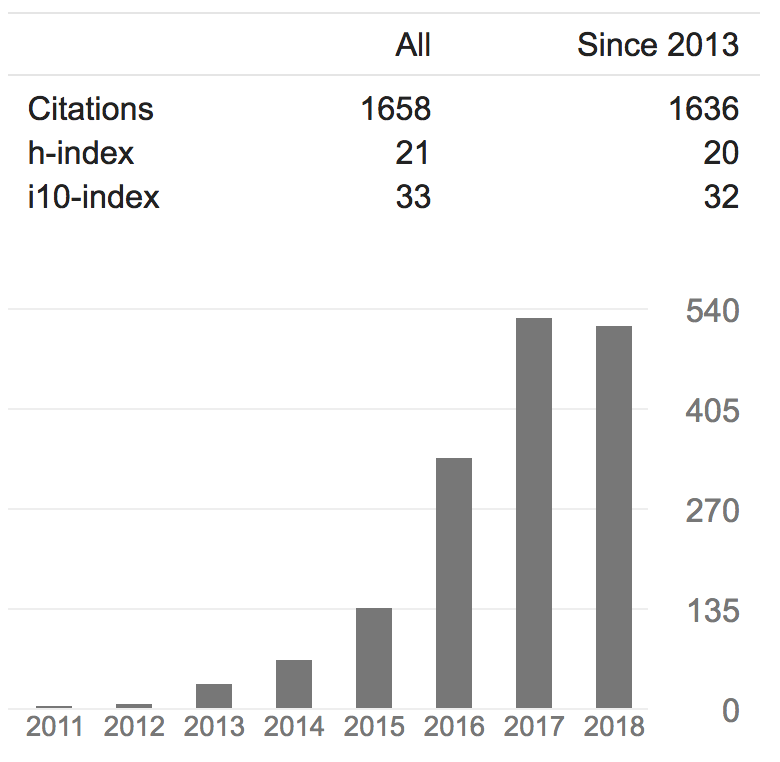
\includegraphics[width=7cm]{screenshot.png}
% \end{figure}
% \section*{DBLP recorded publications}


\nocite{*} 

\medskip

%Filters bibliography
\printbibliography[sorting=ydnt,heading=subbibintoc,type=article,title={Journal Publications}]
%\newrefcontext[sorting=ydnt]
%\printbibliography[type=book,title={Book Editions}]
%\newrefcontext[sorting=ydnt]
%\printbibliography[type=inproceedings,title={Peer-reviewed Conference Papers}]

% \printbibliography[keyword={physics},title={Physics-related only}]
% \printbibliography[keyword={latex},title={\LaTeX-related only}]

\end{document}
